% ===========================================================================
%  PART III --- GENERALIZED ADVANTAGE ESTIMATION (Schulman et al., 2015)
% ===========================================================================
\clearpage
\part{Generalized Advantage Estimation}

\partintro{\textbf{The question of Part III:} TRPO multiplies each ratio by an advantage estimate $\hat A_t$, and Monte Carlo returns make it very noisy. GAE uses a learned \textbf{value function} (the critic) and one knob $\lambda$ to trade \textbf{bias for variance} --- TD($\lambda$), applied to advantages.}

% ---------------------------------------------------------------------------
\section{Where TRPO leaves us}
% ---------------------------------------------------------------------------

\begin{center}
\begin{tikzpicture}[font=\small, >=Stealth,
    q/.style={fl, line width=0.8pt, text width=3.7cm, minimum height=1.05cm}]
  \node[q, cbox=AtlasSlate, text width=9cm] (trpo) at (0,0)
    {\textbf{The TRPO update}\\[2pt]
     $\displaystyle\max_\theta\ \hat\E_t\Big[\frac{\pi_\theta(a_t\mid s_t)}{\pi_{\told}(a_t\mid s_t)}\,{\color{AtlasWarm}\hat A_t}\Big]
       \quad\text{s.t.}\quad {\color{AtlasCool}\bar D_{\mathrm{KL}}(\told,\theta)\le\delta}$};
  \node[q, cbox=AtlasWarm] (adv) at (-4.4,-2.1) {\textbf{\color{AtlasWarm}Where does $\hat A_t$ come from?}\\ Monte Carlo returns:\\ unbiased, \textbf{high variance}};
  \node[q, cbox=AtlasSlate, text=NoteGray] (st) at (0,-2.1) {\textbf{Where do states come from?}\\ $s_0\sim\rho_0$, then $\piold$\\ no $\mu$ (lane B)};
  \node[q, cbox=AtlasCool] (sol) at (4.4,-2.1) {\textbf{\color{AtlasCool}How is it solved?}\\ CG + line search: second order,\\ \textbf{one step} per batch};
  \node[q, cbox=AtlasWarm, fill=AtlasWarm!18] (gae) at (-4.4,-4.3) {\textbf{GAE} (2015)\\ a value function trades\\ bias for variance via $\lambda$};
  \node[q, draw=AtlasSlate!50, dashed, text=NoteGray] (open) at (0,-4.3) {\textbf{still open}\\ neither paper changes\\ where states come from};
  \node[q, cbox=AtlasCool, fill=AtlasCool!18] (ppo) at (4.4,-4.3) {\textbf{PPO} (2017)\\ first order: clip the ratio,\\ $K$ epochs of SGD per batch};
  \draw[->, thick, AtlasWarm] (trpo.south) ++(-2.5,0) -- (adv.north);
  \draw[->, thick, AtlasSlate!60] (trpo.south) -- (st.north);
  \draw[->, thick, AtlasCool] (trpo.south) ++(2.5,0) -- (sol.north);
  \draw[->, thick, AtlasWarm] (adv) -- (gae);
  \draw[->, thick, AtlasSlate!50, dashed] (st) -- (open);
  \draw[->, thick, AtlasCool] (sol) -- (ppo);
\end{tikzpicture}
\end{center}

{\small The update is written as in the GAE paper (Sec.~6.1, Eq.~31). TRPO itself used Monte Carlo $\hat Q$, which differs from an advantage only by a baseline. PPO's intro lists TRPO's other drawbacks: complicated, and incompatible with noise (dropout) or parameter sharing between policy and value.}

% ---------------------------------------------------------------------------
\section{Setting}
% ---------------------------------------------------------------------------

\paper{High-Dimensional Continuous Control Using Generalized Advantage Estimation}
  {Schulman, Moritz, Levine, Jordan \& Abbeel}{ICLR 2016 (arXiv 2015)}
  {GAE$(\gamma,\lambda)$ --- TD($\lambda$) for advantages, plus a trust-region value fit}
  {gae.md}

\begin{enumerate}
  \item Same MDP as TRPO: start distribution $\rho_0$, unknown dynamics, reward $r_t=r(s_t,a_t,s_{t+1})$.
  \item \textbf{Undiscounted} goal: maximize $\E\big[\sum_t r_t\big]$ (assumed finite).
  \item $\gamma$ is \textbf{not part of the problem}: it is an algorithm knob that trades bias for variance.
  \item Any policy-gradient method --- here TRPO for the policy, and a trust region for $V_\phi$ too.
  \item 3D robots, neural nets with $>10^4$ parameters, torques from raw kinematics.
\end{enumerate}

\begin{notebox}
All quantities are unnormalized, like TRPO and unlike CPI. The formula itself appeared earlier (Kimura \& Kobayashi 1998; Wawrzy\'nski 2009); the paper's contribution is the analysis that makes it usable with batch trust-region methods, plus the trust-region value fit.
\end{notebox}

\subsection{What GAE fixes --- and what it does not}

\begin{minipage}[c]{0.5\linewidth}
\centering
\begin{tikzpicture}
\begin{axis}[notes, width=7cm, height=4.4cm, xmin=-1.3, xmax=1.3, ymin=-0.5, ymax=2.5,
    ytick={0,1,2}, yticklabels={$\lambda=0$, $0<\lambda<1$, $\lambda=1$}, xtick={0.3}, xticklabels={true $A$},
    axis lines=box, only marks, mark size=1.8pt]
  \addplot[AtlasSlate, mark=*] coordinates {(-0.9,2)(-0.55,2)(-0.2,2)(0.05,2)(0.3,2)(0.55,2)(0.8,2)(1.1,2)(0.4,2)(-0.1,2)};
  \addplot[AtlasWarm, mark=*] coordinates {(-0.25,1)(-0.05,1)(0.1,1)(0.2,1)(0.3,1)(0.42,1)(0.55,1)(0.65,1)};
  \addplot[AtlasCool, mark=*] coordinates {(-0.45,0)(-0.38,0)(-0.32,0)(-0.27,0)(-0.22,0)(-0.17,0)(-0.12,0)(-0.07,0)};
  \draw[dashed, gray] (axis cs:0.3,-0.5) -- (axis cs:0.3,2.5);
\end{axis}
\end{tikzpicture}\\
{\scriptsize Each dot: one estimate $\hat A_t$ of the same $(s_t,a_t)$ (schematic).}
\end{minipage}\hfill
\begin{minipage}[c]{0.47\linewidth}
\begin{enumerate}
  \item TRPO multiplies each ratio by $\hat A_t$. From one rollout: \textbf{unbiased}, but \textbf{very noisy} (top row).
  \item A learned \textbf{value function} $V$ --- the \emph{critic}: low noise, but \textbf{biased} if $V$ is wrong (bottom row).
  \item $\lambda$ slides between the two: a \textbf{bias--variance knob} (middle row).
\end{enumerate}
\end{minipage}

\begin{pair}
\begin{keybox}[title={Fixes}]
Noisy update directions $\Rightarrow$ fewer samples per step.
\end{keybox}
\begin{warnbox}[title={Not an exploration knob}]
$\lambda$ changes how we \emph{score} sampled actions, not \emph{which states} we visit.
\end{warnbox}
\end{pair}

\begin{notebox}
GAE abstract: two challenges --- ``the large number of samples typically required, and the difficulty of obtaining stable and steady improvement''. Value functions attack the first, a trust region for both policy and value attacks the second. Sec.~1: ``bias is more pernicious --- even with an unlimited number of samples, bias can cause the algorithm to fail to converge.''
\end{notebox}

% ---------------------------------------------------------------------------
\section{Which weight multiplies the score function?}
% ---------------------------------------------------------------------------

All policy-gradient estimators have the same form:
\begin{gather*}
  g = \E\Big[\sum_{t\ge0} \Psi_t\,\nabla_\theta\log\pi_\theta(a_t\mid s_t)\Big]
\end{gather*}

\begin{minipage}[c]{0.5\linewidth}
Same expectation for each choice of $\Psi_t$ --- \textbf{different variance}:\par\vspace{2pt}
\small
\begin{tabular}{r l l}
\toprule
 & $\Psi_t$ & \\
\midrule
1 & $\sum_{t'\ge0} r_{t'}$ & total return \\
2 & $\sum_{t'\ge t} r_{t'}$ & reward after $a_t$ \\
3 & $\sum_{t'\ge t} r_{t'} - b(s_t)$ & with a baseline \\
4 & $Q^\pi(s_t,a_t)$ & action value \\
5 & {\color{AtlasCool}$\boldsymbol{A^\pi(s_t,a_t)}$} & {\color{AtlasCool}\textbf{advantage}} \\
6 & $r_t + V^\pi(s_{t+1}) - V^\pi(s_t)$ & TD residual \\
\bottomrule
\end{tabular}
\end{minipage}\hfill
\begin{minipage}[c]{0.46\linewidth}
\begin{keybox}[title={Why the advantage}]
\begin{itemize}
  \item ``Almost the lowest possible variance'' (Greensmith et al., 2004).
  \item A step along $A\,\nabla\log\pi$ raises $\pi(a\mid s)$ \textbf{iff} $a$ beats the average $V^\pi$ --- the gaps of the Notation figure in Part~I.
\end{itemize}
\end{keybox}
\end{minipage}

\begin{slatebox}[title={The discount as a knob}]
The discounted gradient $g^\gamma$ uses $A^{\pi,\gamma}$, which ignores effects $\gg\frac{1}{1-\gamma}$ steps later $\Rightarrow$ less variance, \textbf{some bias}. An estimator $\hat A_t$ is \emph{$\gamma$-just} if it gives an unbiased estimate of $g^\gamma$ (Def.~1, Prop.~1). From here on, bias means bias \emph{relative to} $g^\gamma$.
\end{slatebox}

% ---------------------------------------------------------------------------
\section{GAE: TD($\lambda$) for advantages}
% ---------------------------------------------------------------------------

Four steps, from one TD residual to all of them.

\begin{enumerate}
  \item \textbf{TD residual} --- one reward, then $V$:
  \begin{gather*}
    \delta_t^V = r_t + \gamma V(s_{t+1}) - V(s_t)
  \end{gather*}
  \item \textbf{$k$ residuals} --- $\hat A_t^{(k)}=\sum_{l<k}\gamma^l\delta_{t+l}^V$ telescopes to
  \begin{gather*}
    \hat A_t^{(k)} = -V(s_t) + \textstyle\sum_{l=0}^{k-1}\gamma^l r_{t+l} + \gamma^k V(s_{t+k})
  \end{gather*}
  \item \textbf{All of them} --- the return minus a baseline:
  \begin{gather*}
    \hat A_t^{(\infty)} = \textstyle\sum_{l\ge0}\gamma^l r_{t+l} - V(s_t)
  \end{gather*}
  \item \textbf{GAE} --- average all $k$ with weights $(1-\lambda)\lambda^{k-1}$:
\end{enumerate}

\begin{eqbox}
\begin{gather*}
  \hat A_t^{\mathrm{GAE}(\gamma,\lambda)} = (1-\lambda)\textstyle\sum_{k\ge1}\lambda^{k-1}\hat A_t^{(k)} = \textstyle\sum_{l\ge0}(\gamma\lambda)^l\,\delta_{t+l}^V
\end{gather*}
\end{eqbox}

\begin{minipage}[c]{0.5\linewidth}
\centering
\begin{tikzpicture}[x=0.85cm, y=0.8cm, >=Stealth,
    st/.style={circle, fill=AtlasSlate, minimum size=0.16cm, inner sep=0pt},
    real/.style={AtlasWarm, line width=2.4pt, line cap=round},
    boot/.style={circle, draw=AtlasWarm, very thick, fill=white, minimum size=0.32cm, inner sep=0pt},
    base/.style={rectangle, draw=AtlasSlate, thick, fill=AtlasSlate!25, minimum size=0.22cm, inner sep=0pt},
    lab/.style={font=\scriptsize, anchor=east}]
  \foreach \i/\n in {0/t, 1/t{+}1, 2/t{+}2, 3/t{+}3, 4/t{+}4} {
    \node[st] (s\i) at (\i,0) {};
    \node[font=\tiny, above=2pt of s\i] {$s_{\n}$};}
  \foreach \i/\j in {0/1, 1/2, 2/3, 3/4} \draw[->, AtlasSlate, shorten <=2pt, shorten >=2pt] (s\i) -- (s\j);
  \node[lab] at (-0.3,-1.0) {$k=1$};
  \node[base] at (0,-1.0) {}; \draw[real] (0.15,-1.0) -- (1,-1.0); \node[boot] at (1,-1.0) {};
  \node[lab] at (-0.3,-1.8) {$k=3$};
  \node[base] at (0,-1.8) {}; \draw[real] (0.15,-1.8) -- (3,-1.8); \node[boot] at (3,-1.8) {};
  \node[lab] at (-0.3,-2.6) {$k=\infty$};
  \node[base] at (0,-2.6) {}; \draw[real] (0.15,-2.6) -- (5.0,-2.6);
  \node[font=\tiny, anchor=west] at (-1.1,-3.4)
    {\tikz\node[base]{}; $-V(s_t)$ \;\; \tikz\draw[real] (0,0) -- (0.35,0); rewards \;\; \tikz\node[boot] {}; $\gamma^kV(s_{t+k})$};
\end{tikzpicture}
\end{minipage}\hfill
\begin{minipage}[c]{0.47\linewidth}
\centering
\begin{tikzpicture}
\begin{axis}[notes, width=6.8cm, height=4.3cm, ybar, bar width=4pt, ymin=0, ymax=0.55,
    xlabel={$k$ (number of residuals)}, xtick={1,...,10}, ytick={0,0.25,0.5},
    legend pos=north east, area legend, title={\small weights $(1-\lambda)\lambda^{k-1}$}]
  \addplot[fill=AtlasCool!70, draw=none] coordinates {(1,0.5)(2,0.25)(3,0.125)(4,0.0625)(5,0.031)(6,0.016)(7,0.008)(8,0.004)(9,0.002)(10,0.001)};
  \addlegendentry{$\lambda=0.5$}
  \addplot[fill=AtlasWarm!70, draw=none] coordinates {(1,0.1)(2,0.09)(3,0.081)(4,0.073)(5,0.066)(6,0.059)(7,0.053)(8,0.048)(9,0.043)(10,0.039)};
  \addlegendentry{$\lambda=0.9$}
\end{axis}
\end{tikzpicture}
\end{minipage}

\begin{center}
\small
\begin{tabular}{l l l}
\toprule
 & $\lambda=0$: \ $\hat A_t=\delta_t^V$ & $\lambda=1$: \ $\hat A_t=\sum_l\gamma^lr_{t+l}-V(s_t)$ \\
\midrule
bias & biased unless $V=V^{\pi,\gamma}$ & unbiased for $g^\gamma$, \textbf{any} $V$ \\
variance & low & high \\
\bottomrule
\end{tabular}
\end{center}

\begin{notebox}
The same picture as TD(0)$\to$Monte Carlo in Part~I: TD($\lambda$) estimates a value, GAE an advantage; the only change is the baseline $-V(s_t)$ at the start of every row. The bias shrinks with $k$ because the bootstrapped term $\gamma^kV(s_{t+k})$ is discounted more, while $-V(s_t)$ never adds bias (it is a baseline).
\end{notebox}

% ---------------------------------------------------------------------------
\section{Two knobs, two kinds of bias}
% ---------------------------------------------------------------------------

\begin{minipage}[c]{0.5\linewidth}
\centering
\begin{tikzpicture}
\begin{axis}[notes, width=7cm, height=4.4cm, xmin=0, xmax=12, ymin=0, ymax=1.25,
    xlabel={delay $l$}, ytick=\empty, xtick={0,4,8,12}, legend pos=north east,
    declare function={raw(\x) = 0.25 + 0.55*exp(-0.18*\x) + 0.12*sin(deg(1.3*\x))*exp(-0.08*\x);
                       shaped(\x) = 1.1*exp(-1.3*\x);}]
  \addplot[draw=none, fill=AtlasWarm!15, forget plot] coordinates {(0,0)(0,1.25)(1.8,1.25)(1.8,0)} \closedcycle;
  \addplot[AtlasSlate, very thick, domain=0:12, samples=100] {raw(x)};
  \addlegendentry{raw reward}
  \addplot[AtlasWarm, very thick, domain=0:12, samples=100] {shaped(x)};
  \addlegendentry{shaped by $V$: $\delta^V$}
\end{axis}
\end{tikzpicture}\\
{\scriptsize $\chi(l;s,a)=\E[r_{t+l}\mid s,a]-\E[r_{t+l}\mid s]$: how long $a_t$ keeps mattering.}
\end{minipage}\hfill
\begin{minipage}[c]{0.47\linewidth}
\begin{pair}[1]
\begin{slatebox}[title={$\gamma$: cut the horizon}]
\small Drops effects after $\approx\frac{1}{1-\gamma}$ steps. Biased \textbf{even with the exact} $V$.
\end{slatebox}
\begin{warmbox}[title={$\lambda$: shape, then cut again}]
\small $\delta^V$ is the reward \emph{shaped} by $\Phi=V$: a good $V$ pulls the effect of $a_t$ to $l\approx0$. Biased \textbf{only if $V$ is wrong}.
\end{warmbox}
\end{pair}
\end{minipage}

\begin{keybox}
So the best $\lambda$ is \textbf{lower} than the best $\gamma$ (numbers in \S\ref{sec:gae-results}).
\end{keybox}

\begin{notebox}
\textbf{Reward shaping} (Ng et al., 1999): $\tilde r=r+\gamma\Phi(s')-\Phi(s)$ leaves $A^{\pi,\gamma}$ unchanged. With $\Phi=V$ it is exactly $\delta^V$, and GAE is the $(\gamma\lambda)$-discounted sum of shaped rewards (Eq.~20). With $\Phi=V^{\pi,\gamma}$ the shaped response is nonzero only at $l=0$. Response function: $A^{\pi,\gamma}(s,a)=\sum_l\gamma^l\chi(l;s,a)$ (Eq.~22). The curves are illustrative.
\end{notebox}

% ---------------------------------------------------------------------------
\section{Actor--critic: policy and value networks}
% ---------------------------------------------------------------------------

\begin{minipage}[c]{0.5\linewidth}
\centering
\begin{tikzpicture}[font=\scriptsize, >=Stealth,
    ac/.style={fl, line width=0.8pt, text width=2.7cm, minimum height=0.9cm, font=\scriptsize}]
  \node[ac, cbox=AtlasSlate] (env) at (0,0) {\textbf{1. Rollouts}\\ run $\pi_{\theta_i}$ for $N$ steps};
  \node[ac, cbox=AtlasWarm] (crit) at (1.85,-1.85) {\textbf{\color{AtlasWarm}2. Critic $V_{\phi_i}$}\\ $\delta_t^V$, \ $\hat A_t=\sum_l(\gamma\lambda)^l\delta_{t+l}^V$};
  \node[ac, cbox=AtlasCool] (act) at (-1.85,-1.85) {\textbf{\color{AtlasCool}3. Actor $\pi_\theta$}\\ TRPO step with $\hat A_t$};
  \node[ac, cbox=AtlasWarm, fill=AtlasWarm!18] (fit) at (1.85,-3.6) {\textbf{4. Fit the critic}\\ regression, trust region $\to\phi_{i+1}$};
  \draw[->, thick, AtlasSlate] (env) -- (crit);
  \draw[->, thick, AtlasSlate] (crit) -- node[above, font=\tiny]{$\hat A_t$} (act);
  \draw[->, thick, AtlasSlate] (crit) -- (fit);
  \draw[->, thick, AtlasSlate] (act) -- node[left, font=\tiny]{$\theta_{i+1}$} (env);
\end{tikzpicture}
\end{minipage}\hfill
\begin{minipage}[c]{0.47\linewidth}
\begin{itemize}
  \item \textbf{Actor}: the policy network, updated by TRPO.
  \item \textbf{Critic}: a second network $V_\phi(s)\approx V^{\pi,\gamma}(s)$, fitted by regression to Monte Carlo returns $\hat V_n=\sum_l\gamma^lr_{n+l}$.
  \item \textbf{Order matters}: fit $V$ \emph{after} computing $\hat A_t$ --- an overfit $V$ makes every $\delta_t^V=0$.
\end{itemize}
\end{minipage}

\begin{warmbox}[title={Value fit with a trust region}]
\begin{gather*}
  \min_\phi\ \sum_n \big\|V_\phi(s_n) - \hat V_n\big\|^2
  \quad \text{s.t.}\ \ \frac1N\sum_n \frac{\|V_\phi(s_n) - V_{\phi_{\mathrm{old}}}(s_n)\|^2}{2\sigma^2} \le \epsilon
\end{gather*}
\begin{itemize}
  \item $=$ a KL trust region for a Gaussian with mean $V_\phi(s)$; $\sigma^2$ is the current mean squared error.
  \item Solved with conjugate gradient, like TRPO.
  \item Keeps $V$ from overfitting the latest batch --- the ``stable improvement'' challenge of the abstract.
\end{itemize}
\end{warmbox}

\begin{notebox}
Unlike Q-learning-style critics (e.g.\ SAC, which learns $Q(s,a)$ off-policy), GAE's critic is a state value $V(s)$ fitted \textbf{on-policy}. Networks: three hidden layers (100, 50, 25 tanh units) for both policy and value. TD($\lambda$) targets for the critic made no difference.
\end{notebox}

% ---------------------------------------------------------------------------
\section{Results: choosing $\gamma$ and $\lambda$}
\label{sec:gae-results}
% ---------------------------------------------------------------------------

\begin{minipage}[c]{0.56\linewidth}
\centering
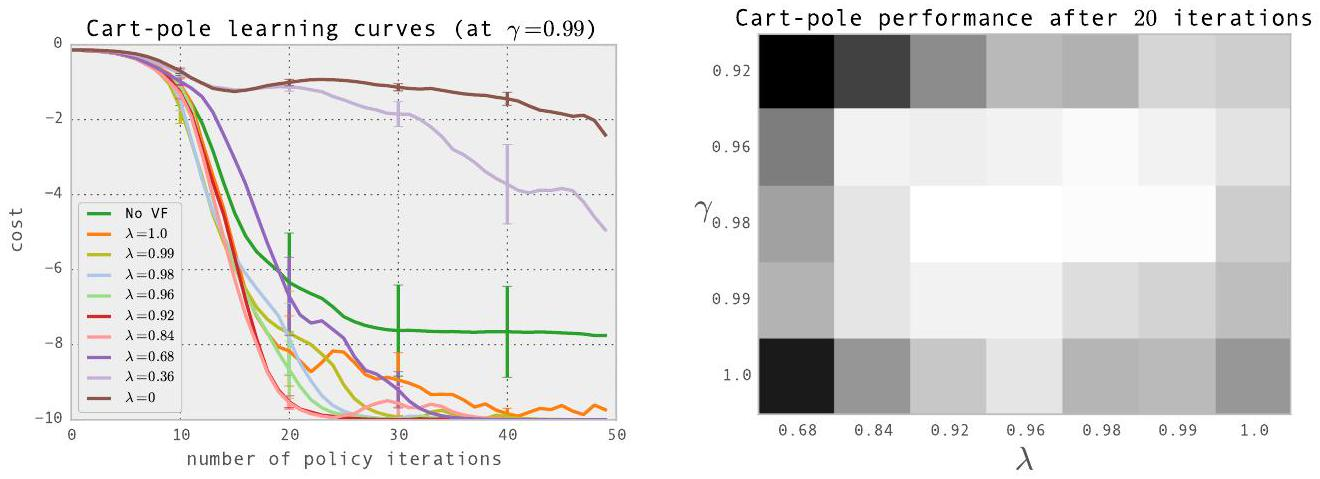
\includegraphics[width=\linewidth]{gae_fig2_sweep.jpg}\\[2pt]
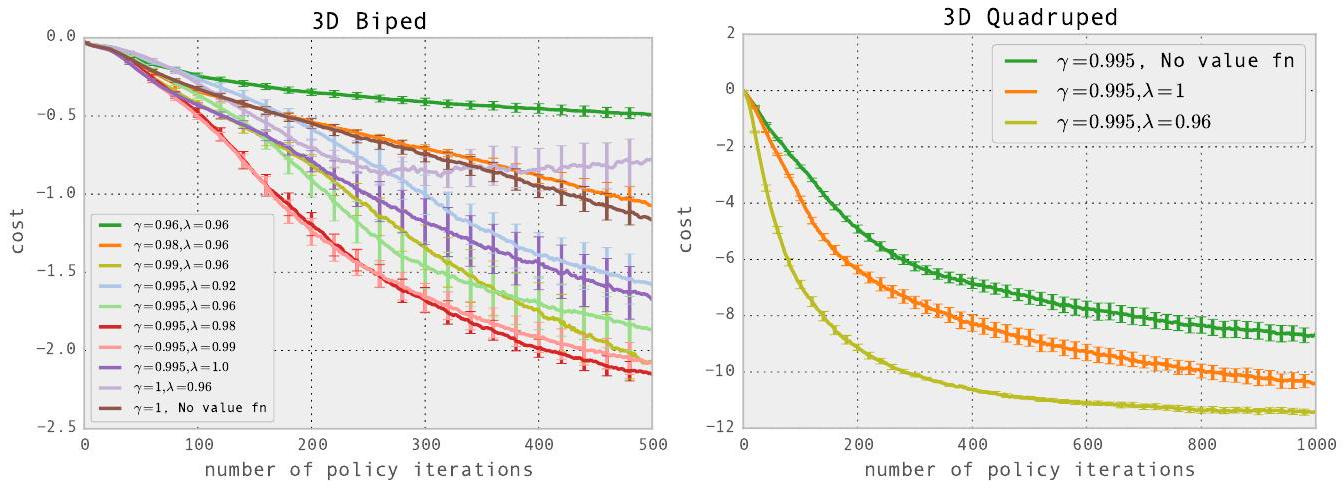
\includegraphics[width=\linewidth]{gae_fig3_3d.jpg}\\
{\scriptsize GAE Figs.~2--3. Cost $=$ negative reward (lower is better).}
\end{minipage}\hfill
\begin{minipage}[c]{0.41\linewidth}
\textbf{Cart-pole} (top)
\begin{itemize}
  \item best at intermediate $\lambda\in[0.92,0.99]$, $\gamma\in[0.96,0.99]$
  \item $\lambda=0$ and ``No VF'' (time-dependent baseline only) much worse
\end{itemize}
\textbf{3D biped, quadruped} (bottom)
\begin{itemize}
  \item best $\gamma\in[0.99,0.995]$, $\lambda\in[0.96,0.99]$
  \item the biped runs after 1000 iterations $\approx$ 5.8 days of simulated time
\end{itemize}
\end{minipage}

\begin{keybox}
Best $\lambda$ $<$ best $\gamma$: $\lambda$ adds bias only if $V$ is wrong. Discussion: $\lambda\in[0.9,0.99]$ usually best; App.~A.2: the $\lambda=0$ estimator was ``prohibitively'' biased.
\end{keybox}
